\subsection{x86}

\myindex{x86!\Instructions!LOOP}

There is a special \LOOP instruction in x86 instruction set for checking the value in register \ECX and 
if it is not 0, to \gls{decrement} \ECX
and pass control flow to the label in the \LOOP operand. 
Probably this instruction is not very convenient, and there are no any modern compilers which emit it automatically.
So, if you see this instruction somewhere in code, it is most likely that this is a manually written piece 
of assembly code.

\par

In \CCpp loops are usually constructed using \TT{for()}, \TT{while()} or \TT{do/while()} statements.

Let's start with \TT{for()}.
\myindex{\CLanguageElements!for}

This statement defines loop initialization (set loop counter to initial value), 
loop condition (is the counter bigger than a limit?), what is done at each iteration (\gls{increment}/\gls{decrement})
and of course loop body.

\lstinputlisting{patterns/09_loops/simple/loops_1.c.\LANG}

The generated code is consisting of four parts as well.

Let's start with a simple example:

\lstinputlisting[label=loops_src]{patterns/09_loops/simple/loops_2.c}

Result (MSVC 2010):

\lstinputlisting[caption=MSVC 2010]{patterns/09_loops/simple/1_MSVC.asm.\LANG}

As we see, nothing special.

\ifdefined\IncludeGCC

GCC 4.4.1 emits almost the same code, with one subtle difference:

\lstinputlisting[caption=GCC 4.4.1]{patterns/09_loops/simple/1_GCC.asm.\LANG}

Now let's see what we get with optimization turned on (\TT{\Ox}):
\fi

\lstinputlisting[caption=\Optimizing MSVC]{patterns/09_loops/simple/1_MSVC_Ox.asm}

What happens here is that space for the $i$ variable is not allocated in the local stack anymore,
but uses an individual register for it, \ESI.
This is possible in such small functions where there aren't many local variables.

One very important thing is that the \ttf function must not change the value in \ESI.
Our compiler is sure here. 
And if the compiler decides to use the \ESI register in \ttf too, its value would have to be saved 
at the function's prologue and restored at the function's epilogue,
almost like in our listing: please note \TT{PUSH ESI/POP ESI}
at the function start and end.

\ifdefined\IncludeGCC

Let's try GCC 4.4.1 with maximal optimization turned on (\Othree option):

\lstinputlisting[caption=\Optimizing GCC 4.4.1]{patterns/09_loops/simple/1_GCC_O3.asm}

\myindex{Loop unwinding}

Huh, GCC just unwound our loop.

\Gls{loop unwinding} has an advantage in the cases when there aren't much iterations and 
we could cut some execution time by removing all loop support instructions. 
On the other side, the resulting code is obviously larger.

Big unrolled loops are not recommended in modern times, because bigger functions
may require bigger cache footprint%
%
\footnote{A very good article about it: \cite{DrepperMemory}.
Another recommendations about loop unrolling from Intel are here: 
\cite[3.4.1.7]{IntelOptimization}.}.

OK, let's increase the maximum value of the $i$ variable to 100 and try again. GCC does:

\lstinputlisting[caption=GCC]{patterns/09_loops/simple/2_GCC.asm.\LANG}

It is quite similar to what MSVC 2010 with optimization (\Ox) produce, 
with the exception that the \EBX register is allocated for the $i$ variable.

GCC is sure this register will not be modified inside of the \ttf function, 
and if it will, it will be saved at the function prologue and restored at epilogue, 
just like here in the \main function.
\fi

\ifdefined\IncludeOlly
\clearpage
\subsection{x86: \olly}
\myindex{\olly}

Let's compile our example in MSVC 2010 with \Ox and \Obzero 
options and load it into \olly.

It seems that \olly is able to detect simple loops and show them in square brackets, for convenience:

\begin{figure}[H]
\centering
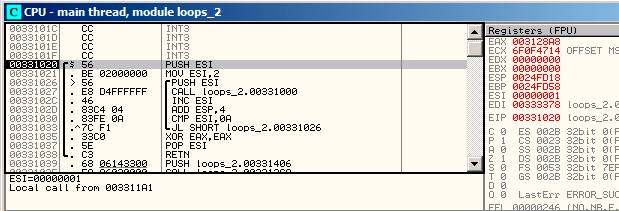
\includegraphics[scale=\FigScale]{patterns/09_loops/simple/olly1.png}
\caption{\olly: \main begin}
\label{fig:loops_olly_1}
\end{figure}

By tracing (F8~--- \stepover) we see \ESI 
\glslink{increment}{incrementing}.
Here, for instance, $ESI=i=6$:

\begin{figure}[H]
\centering
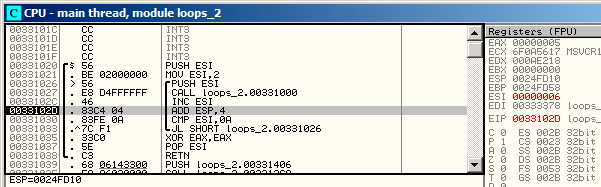
\includegraphics[scale=\FigScale]{patterns/09_loops/simple/olly2.png}
\caption{\olly: loop body just executed with $i=6$}
\label{fig:loops_olly_2}
\end{figure}

9 is the last loop value.
That's why \JL is not triggering after the \gls{increment}, and the function will finish:

\begin{figure}[H]
\centering
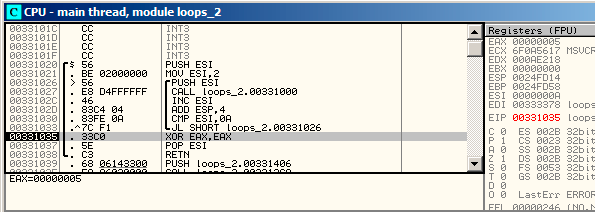
\includegraphics[scale=\FigScale]{patterns/09_loops/simple/olly3.png}
\caption{\olly: $ESI=10$, loop end}
\label{fig:loops_olly_3}
\end{figure}

\subsection{x86: tracer}
\myindex{tracer}

As we might see, it is not very convenient to trace manulally in the debugger.
That's a reason we will try \tracer.

We open compiled example in \IDA, find the address of the instruction \INS{PUSH ESI}
(passing the sole argument to \ttf,) which is \TT{0x401026} for this case and we run the \tracer:

\begin{lstlisting}
tracer.exe -l:loops_2.exe bpx=loops_2.exe!0x00401026
\end{lstlisting}

\TT{BPX} just sets a breakpoint at the address and tracer will then print the state of the registers.

In the \TT{tracer.log} This is what we see:

\lstinputlisting{patterns/09_loops/simple/tracer.log}

We see how the value of \ESI register changes from 2 to 9.

Even more than that, the \tracer can collect register values for all addresses within the function.
This is called \IT{trace} there.
Every instruction gets traced, all interesting register values are recorded.

Then, an \IDA .idc-script is generated, that adds comments.
So, in the \IDA we've learned that the \main function address is \TT{0x00401020} and we run:

\begin{lstlisting}
tracer.exe -l:loops_2.exe bpf=loops_2.exe!0x00401020,trace:cc
\end{lstlisting}

\TT{BPF} stands for set breakpoint on function.

As a result, we get the \TT{loops\_2.exe.idc} and \TT{loops\_2.exe\_clear.idc} scripts.

\clearpage
We load \TT{loops\_2.exe.idc} into \IDA and see:

\begin{figure}[H]
\centering
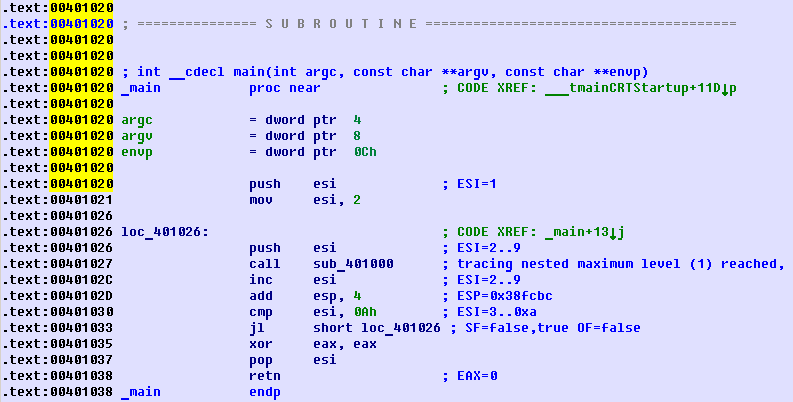
\includegraphics[scale=\FigScale]{patterns/09_loops/simple/IDA_tracer_cc.png}
\caption{\IDA with .idc-script loaded}
\label{fig:loops_IDA_tracer}
\end{figure}

We see that \ESI can be from 2 to 9 at the start of the loop body,
but from 3 to 0xA (10) after the increment.
We can also see that \main is finishing with 0 in \EAX.

\tracer also generates \TT{loops\_2.exe.txt}, 
that contains information about how many times each instruction was executed and
register values:

\lstinputlisting[caption=loops\_2.exe.txt]{patterns/09_loops/simple/loops_2.exe.txt}
\myindex{\GrepUsage}
We can use grep here.

\fi
